\begin{exercise}
\label{ex:03-circumbilliard} 
Show that every triangle has a circumbilliard, i.e., an ellipse to which it is inscribed and to which it is a billiard 3-periodic. Compute the axes of said circumbilliard with respect to triangle vertices. 
\end{exercise}
 
\begin{exercise}
 \label{ex:03-power-euler} 
Prove that the power of the circumcircle with with respect to the common center in each of the following 3-periodic families is constant and given by the listed expressions. (i) incircle: $-a_e b_e$; (ii) homothetic: $-({a_e^2+b_e^2})/{2}$, and (iii) excentral: $-a^2-b^2-2\delta$. 
\end{exercise}

%\begin{exercise}\label{ex:33} 
%The {\em cosine circle} (also known as the second Lemoine circle) \cite[Cosine Circle]{mw} of a triangle passes through 6 points: the 3 pairs of intersections of sides with lines drawn through the symmedian $X_6$ parallel to sides of the orthic triangle. Recall that the orthic vertices are the feet of altitudes. Its center is $X_6$ \cite[Cosine Circle]{mw}. If one takes the excentral triangle of a billiard orbit as the reference triangle,   its orthic is the orbit itself.

%Show that the cosine circle of the excentral triangle is invariant over the family of 3-periodic orbits. Its radius $r^*=(a^2-b^2)/\sqrt{2\delta-a^2-b^2}$ is constant and it is concentric and external to the elliptic billiard.
%\end{exercise}

\begin{exercise}
\label{ex:03-cosine-circle}
Prove the radius $r^*$ of the stationary cosine circle of the excentral family is larger than the major axis $a$ of its caustic. 
\end{exercise}

\begin{exercise}
Show that (i) the cosine circle (also known as the second Lemoine circle) to Brocard porism triangles is stationary, (ii) and that above a certain caustic aspect ratio $a'/b'$, it is tangent to the caustic at two distinct points (below this threshold the caustic is interior to the cosine circle).
\end{exercise}

\begin{exercise}
Show that the first Lemoine circle is stationary over the Brocard porism.
\end{exercise}

\begin{exercise}
A ``third'' Lemoine circle  is defined in \cite{darij2012-ehrmann}. Prove this circle is also stationary over the Brocard porism. 
\end{exercise}

\begin{exercise}
Show that over the poristic family, the locus of the foci of the $X_9$-centered circumconic (the circumbilliard) is a circle.
\end{exercise}

\begin{exercise}
Prove \cref{prop:03-antiorthic}. Furthermore, prove the intersection point of $X_1 X_3$ with the antiorthic axis is the Schöder point $X_{1155}$.
\end{exercise}

\begin{exercise}
A pair of circles uniquely defines a {\em pencil} of coaxial circles; see \cite[Limiting Points]{mw}. The pencil contains exactly two circles which degenerate to a point, known as {\em limiting points}. Derive the location of such points for the poristic pair obtained from the image of two confocal ellipses centered at $[0,0]$ and with axes $a,b$ and $a',b'$.
\end{exercise}

\begin{exercise}
Let $\ell_1,\ell_2$ be the limiting points of the two circles which are polar images of a confocal pair $\E,\E'$ with respect to a circle centered on $f_1$. At what aspect ratio $a/b$ of $\E$ will $\ell_2$ coincide with $f_2$?
\end{exercise}

\begin{exercise}
A well-known result is that the inversion of a circle pair $\C,\C'$ with respect to a circle $\C_1$ centered on $\ell_1$ (resp. $\C_2$ centered on $\ell_2$) is a pair of concentric circles $\C_1'$ and $\C_1''$ (resp. $\C_1'$ and $\C_1''$). Prove the following lesser known result: the ratio of radii between $\C_1'$ and $\C_1''$ is the same as the ratio between $\C_2'$ and $\C_2''$. 
\end{exercise}

\begin{exercise}
Referring to \cref{fig:03-concentric-inverted}, let $\C,\C'$ be the pair of circles which are the polar image of a confocal pair of ellipses $\E,\E'$. Let $\C_1', \C_1''$ be the inversive images of $\C,\C'$ wrt to a cirlce centered on a focus of the ellipse pair. Prove that: (i) $\C_1'$ and $\C_1''$ are concentric with the ellipse pair and (ii) $\C_1'$ (resp. $\C_1''$) is externally tangent to $\E$ (resp. $\E'$) at its left and right major vertices.
\end{exercise}

\begin{figure}
    \centering
    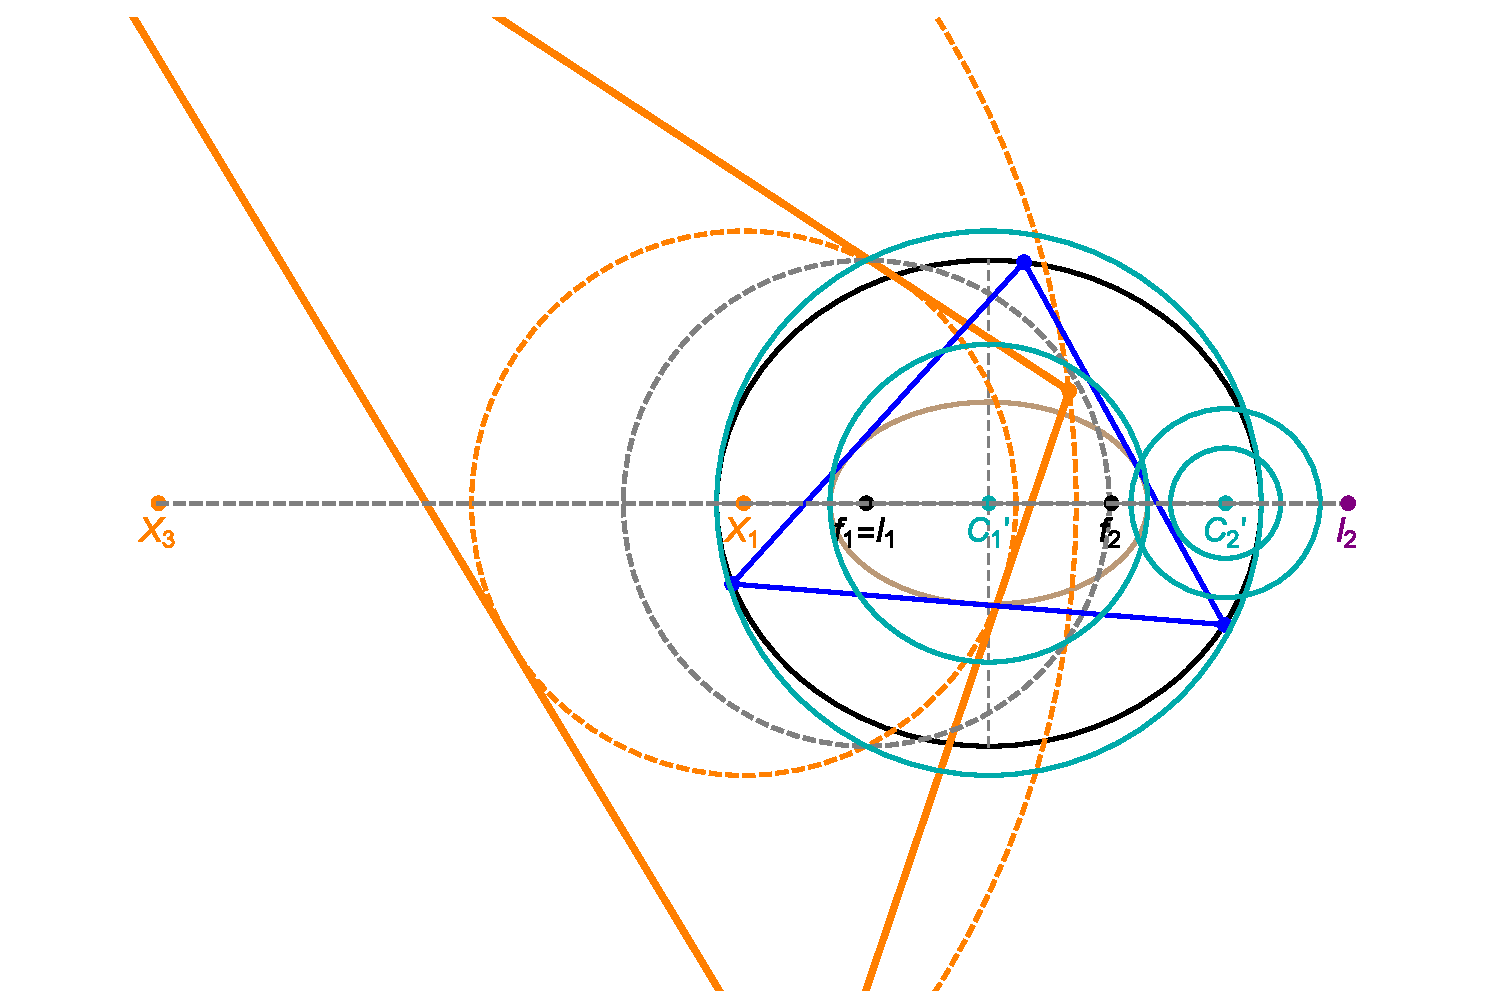
\includegraphics[width=.8\textwidth]{pics_03_210_concentric_inverted_pairs.eps}
    \caption{Caption}
    \label{fig:03-concentric-inverted}
\end{figure}

\begin{exercise}
Prove \cref{lem:03-circum-x5-locus}.
\label{ex:03-circum-x5-locus}
\end{exercise}

\begin{exercise}
Recall the dual family has stationary orthocenter $X_4$. Prove that the inversive image of the dual family wrt to a circle concentric with the ellipse pair is a non-Ponceletian family with incenter $X_1'$ stationary at the common center. This inversive family is inscribed in Booth's curve and its caustic can contain multiple spikes; see it \href{https://bit.ly/3vCCe05}{Live}.
\end{exercise}

\begin{exercise}
Prove the inversive image of billiard 3-periodics with respect to a focus-centered circle is a non-Ponceletian family inscribed in Pascal's Limaçon whose Gergonne point $X_7$ is stationary; see it \href{https://bit.ly/3edwKD7}{Live}. Indeed, this family has constant perimeter (to be shown later).
\end{exercise}

\begin{exercise}
Show that the poristic excentral family is also the polar image of billiard excentrals wrt to a circle centered on a billiard (i.e., the caustic) focus. See it \href{https://bit.ly/33c1s9A}{Live}.
\end{exercise}